\subsection{Evaluation of BHH formula}
The value for $\beta$ differs strongly from area to area, as expected: some areas have a estimated $\beta$ as low as 1.5, while others have $\beta$ close to 6.
These results are tabulated in Table \ref{tab:results}.
It is found that fitting Equation \ref{eq:beardwood} yields a Mean Absolute Percentage error of about 6.8\%, over all observations together, when
letting $\beta$ differ per neighborhood ("Average" row in Table \ref{tab:results}).
When $\beta$ is restricted to be equal for all neighborhoods ("Total row in Table \ref{tab:results}"), this MAPE increases to above 22\%.
The prediction accuracy differs vastly per neighborhood: the Mean Absolute Percentage Error is below 4\% for some areas, and above 18\% for others
(using their own $\beta$).
Potential reasons can best be analyzed using some of the visualizations that were created.

For example, the accuracy for the Schepenbuurt quarter in Friesland, and the Stad van de Zon quarter in Noord-Holland is
especially bad. These areas, among more examples, have an important feature in common. In these quarters, there is a cluster of
addresses somewhere in the area, and another cluster of addresses somewhere else, with empty space between them, as can be seen in Figure \ref{fig:combined}.
Schepenbuurt has a large cluster in the bottom left, with some addresses spread out over the rest of the area. A similar pattern holds for Stad van de Zon.
\begin{figure}[H]
	\centering
	\begin{subfigure}[b]{0.473\textwidth}
		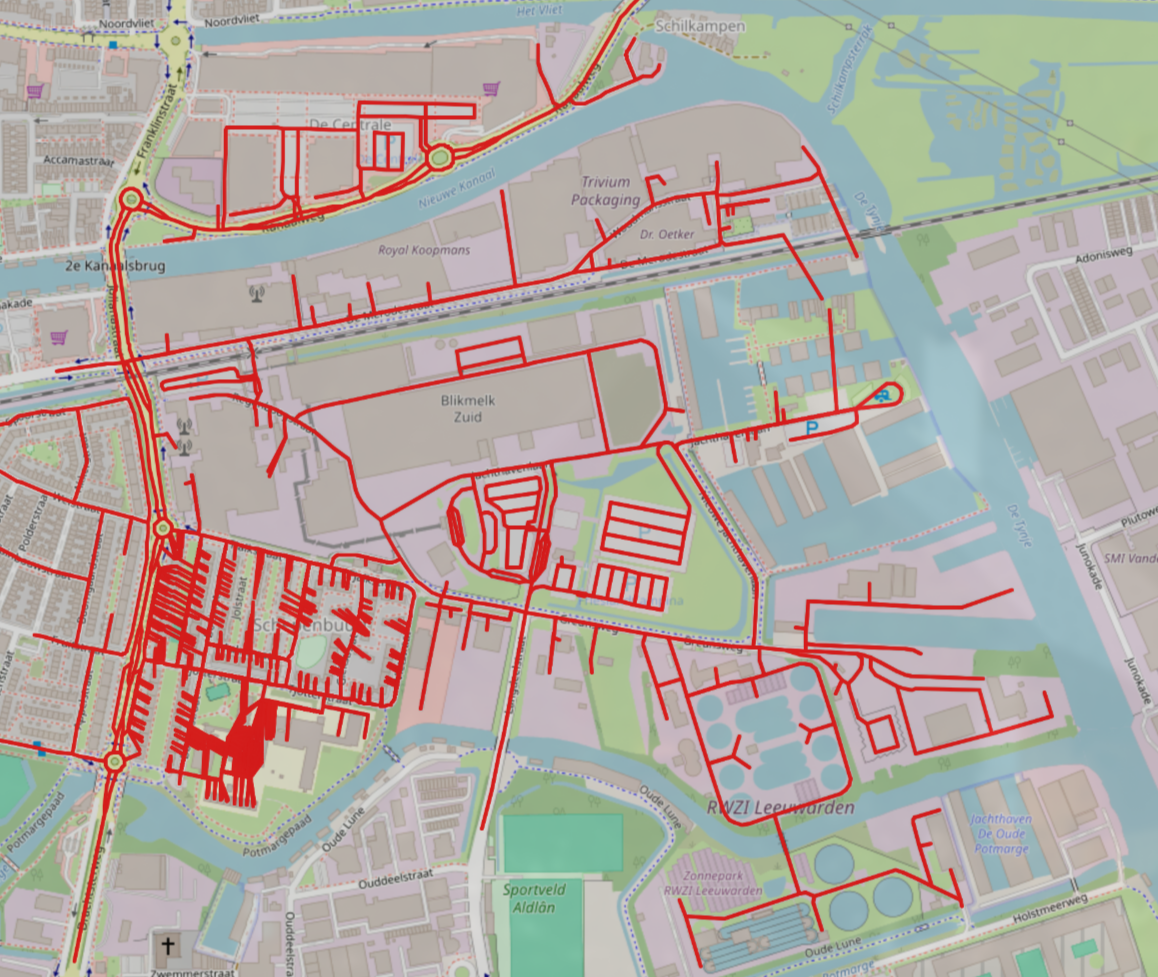
\includegraphics[width=\textwidth]{Pictures/Schepenbuurt_quarter.png}
		\caption{Schepenbuurt}
		\label{fig:Schepenbuurt}
	\end{subfigure}
	\hfill
	\begin{subfigure}[b]{0.49\textwidth}
		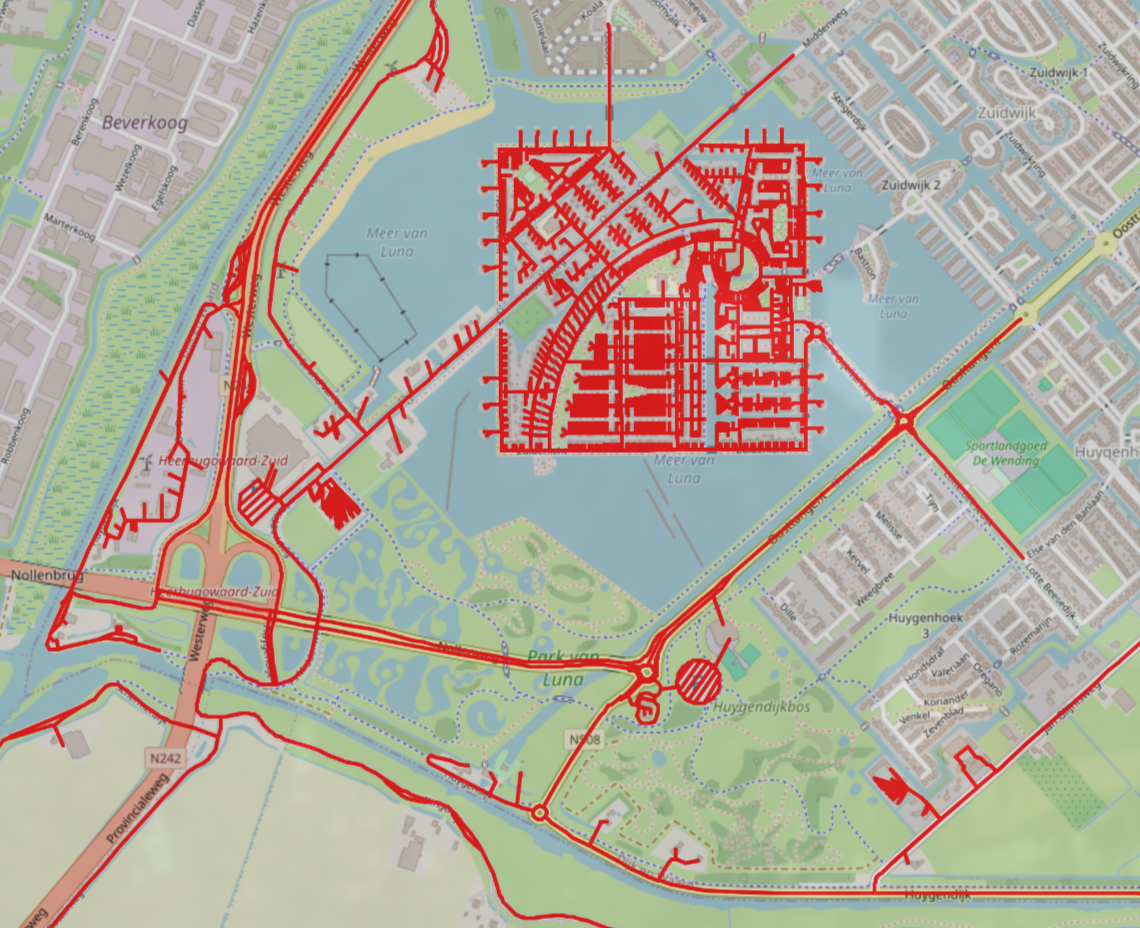
\includegraphics[width=\textwidth]{Pictures/Stad_van_de_Zon_quarter.png}
		\caption{Stad van de Zon}
		\label{fig:StadvdZon}
	\end{subfigure}
	\caption{Maps of the quarters Schepenbuurt and Stad van de Zon.}
	\label{fig:combined}
\end{figure}
An explanation for the higher prediction errors is that when the number of locations to visit $j$ is small, and (as in these examples) one of the clusters is much smaller than
the other, in the sense of number of addresses in it, that there is a significant probability that no addresses in the smaller cluster are in the TSP.
This would result in a significantly lower path length, as the distance to the other cluster and back does not need to be traveled. But, there is also
significant probability that there are addresses of the smaller cluster in the TSP, which would in turn lead to a significantly higher path length.
Based on this, a higher variation in the TSP path length is to be expected, which explains the higher prediction error. This problem would likely disappear when
$j$ is large enough, since then always locations from the other clusters would be chosen as well.

This pattern is again implied by the visualizations in Figure \ref{fig:combinedScatter}. It can be seen especially well for the Stad van de Zon scatter plot,
that there are two separate clusters in the data points. There is a cluster of points far below the fitted line for the BHH formula, and a cluster of points far above it.
As $j$ increases, the amount of data points in the lower cluster decreases. Both of these observations imply these data points are for a TSP that contains locations
only in the large cluster, since the probability of this happening decreases with $j$.
\begin{figure}[H]
	\centering
	\begin{subfigure}[b]{0.49\textwidth}
		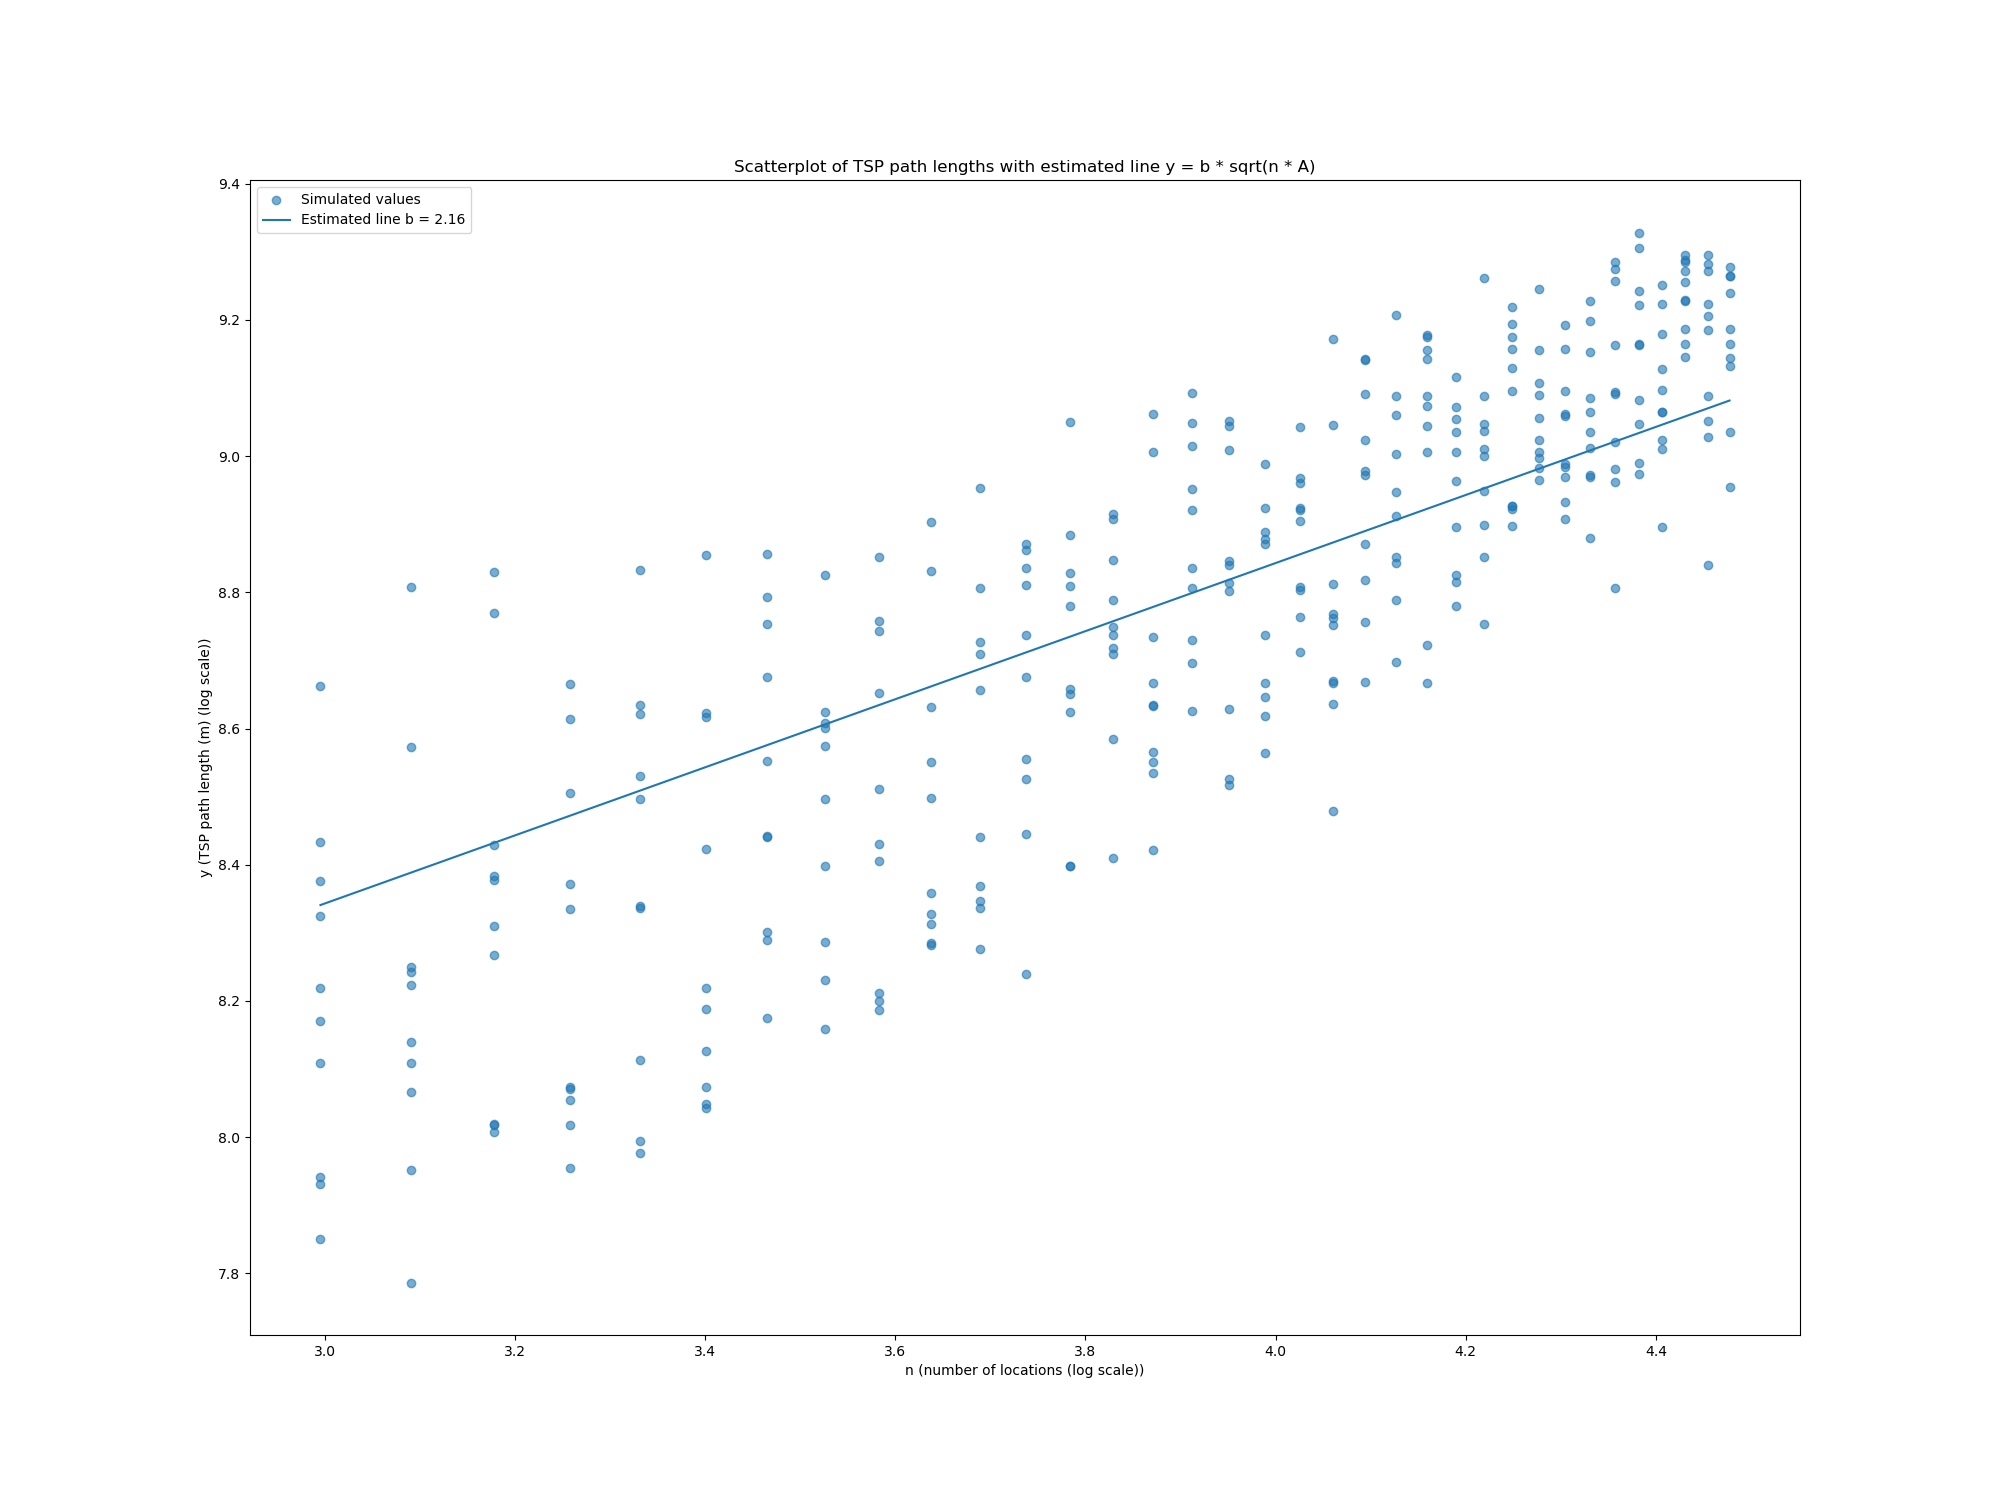
\includegraphics[width=\textwidth]{../project/plots/scatter_friesland-Schepenbuurt.png}
		\caption{Schepenbuurt}
		\label{fig:SchepenbuurtScatter}
	\end{subfigure}
	\hfill
	\begin{subfigure}[b]{0.49\textwidth}
		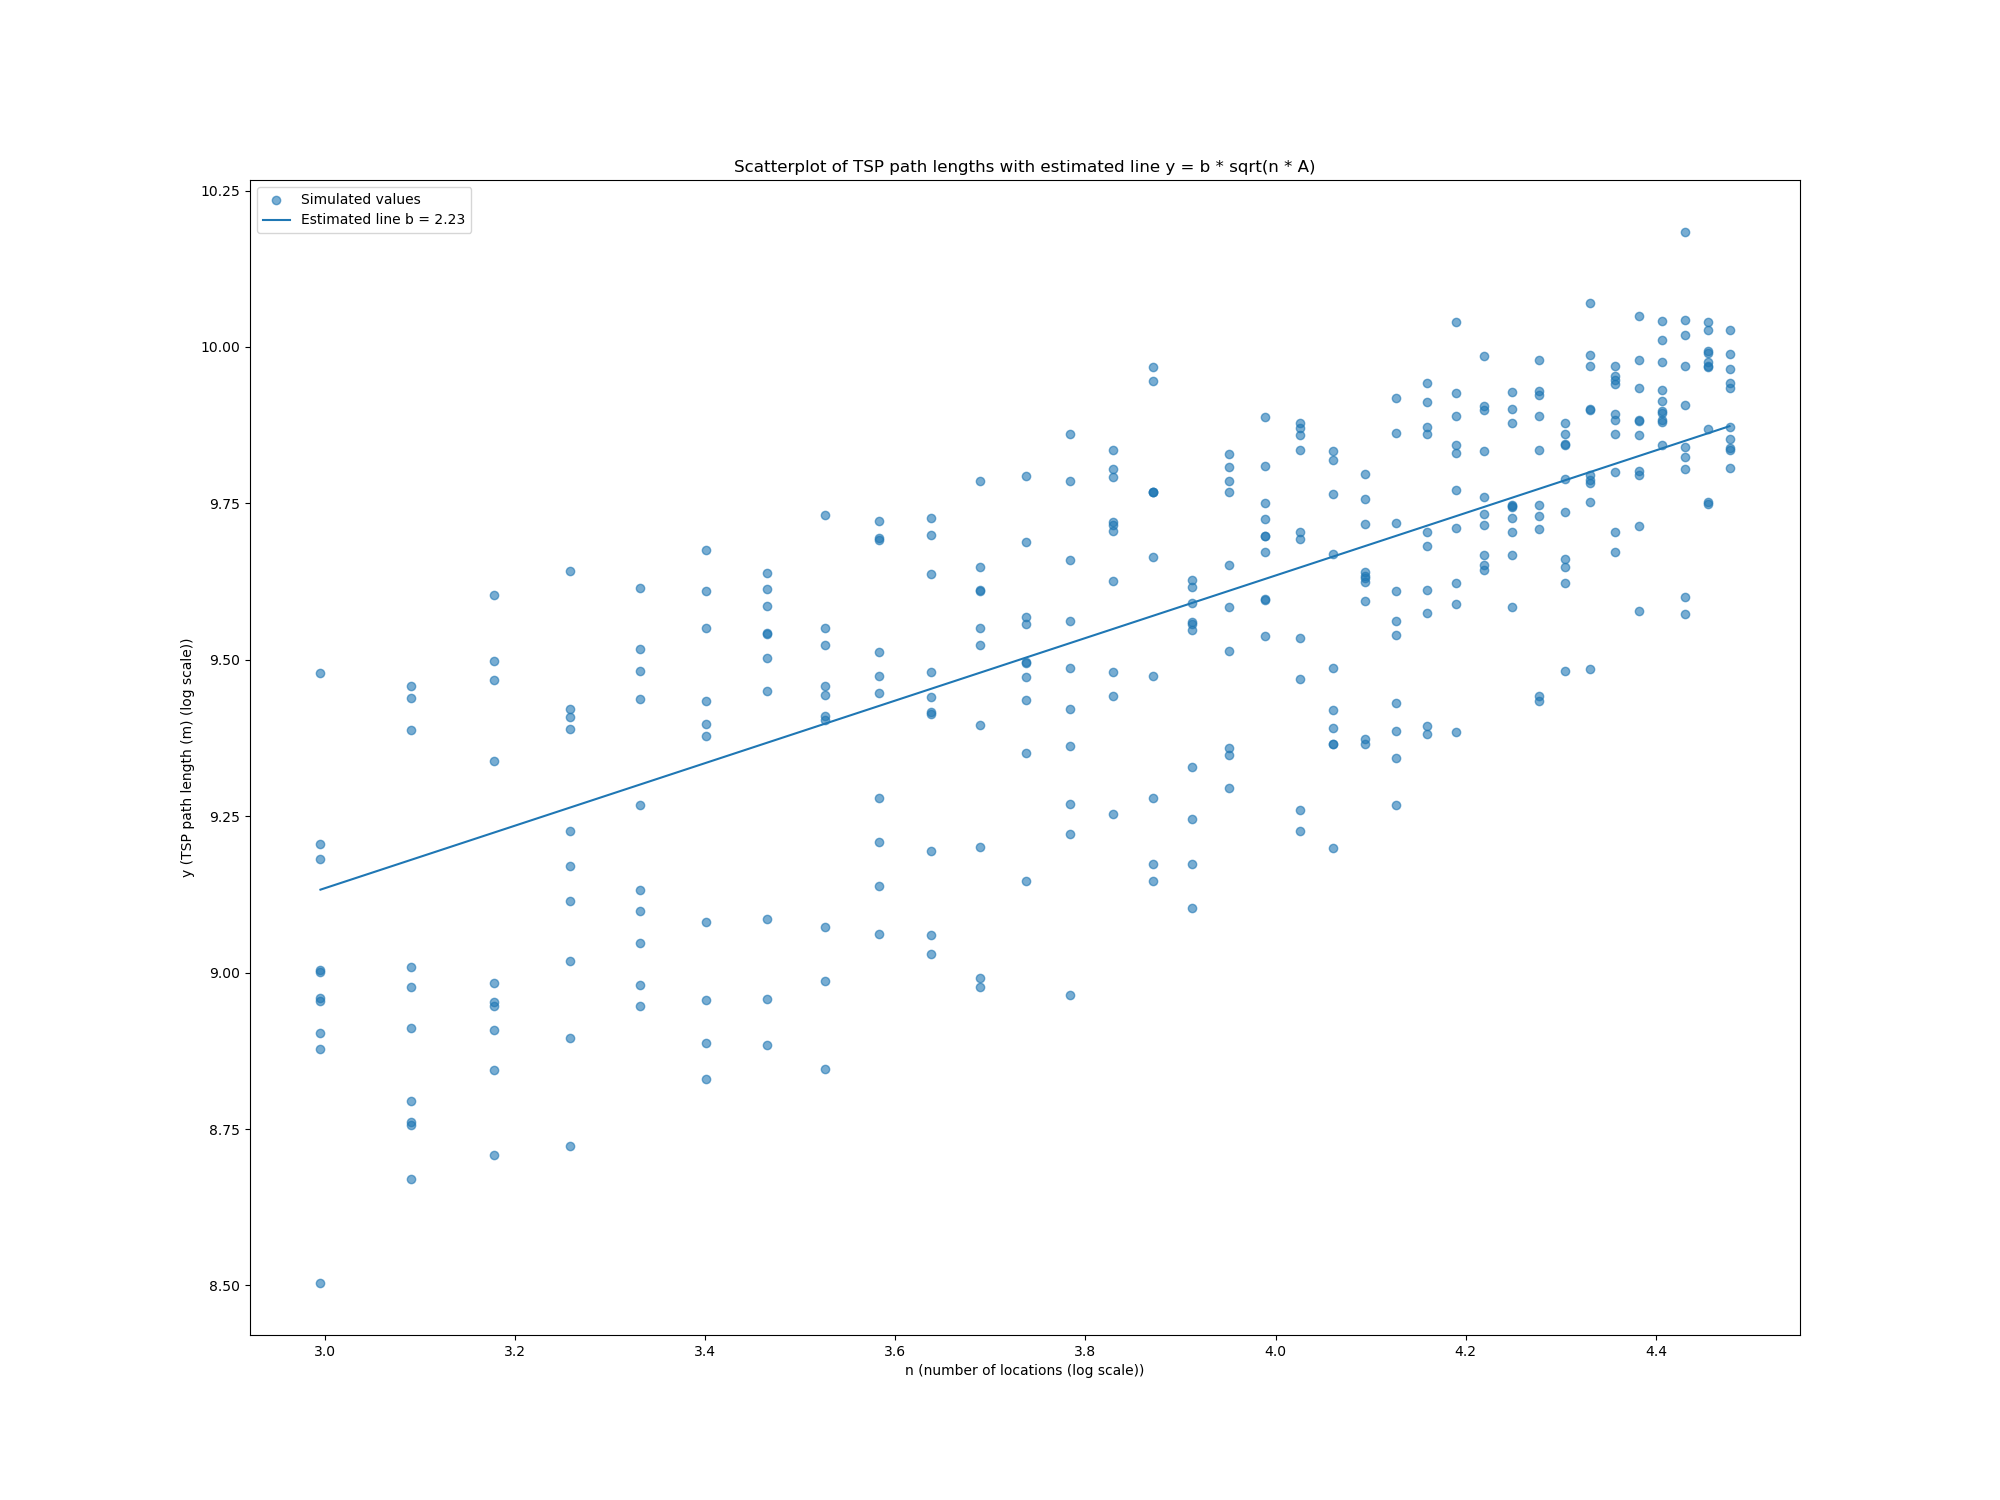
\includegraphics[width=\textwidth]{../project/plots/scatter_noord_holland-Stad van de Zon.png}
		\caption{Stad van de Zon}
		\label{fig:StadvdZonScatter}
	\end{subfigure}
	\caption{Scatter plots of TSP path length vs number of locations for the quarters Schepenbuurt and Stad van de Zon (log-log scale).}
	\label{fig:combinedScatter}
\end{figure}

It is also interesting to consider neighborhoods where the approximations perform especially well. Figure \ref{fig:combined2} displays maps for two quarters,
Westeinde in Friesland and Bornholm in Noord-Holland. These two neighborhoods also share some features. The most important one is that the addresses seem
distributed close to uniformly across the area. There are some 'clusters', for example Westeinde can visually be split into four clusters that are only
connected by one or two main road connections. However, they all contain a large amount of addresses, so each TSP will likely visit all of them. Additionally,
these clusters are all close to each other, there is not much empty space between them, apart from some small greenspace or water. This could explain why the
formula works so much better for these areas, compared to Schepenbuurt and Stad van de Zon.
\begin{figure}[H]
	\centering
	\begin{subfigure}[b]{0.4\textwidth}
		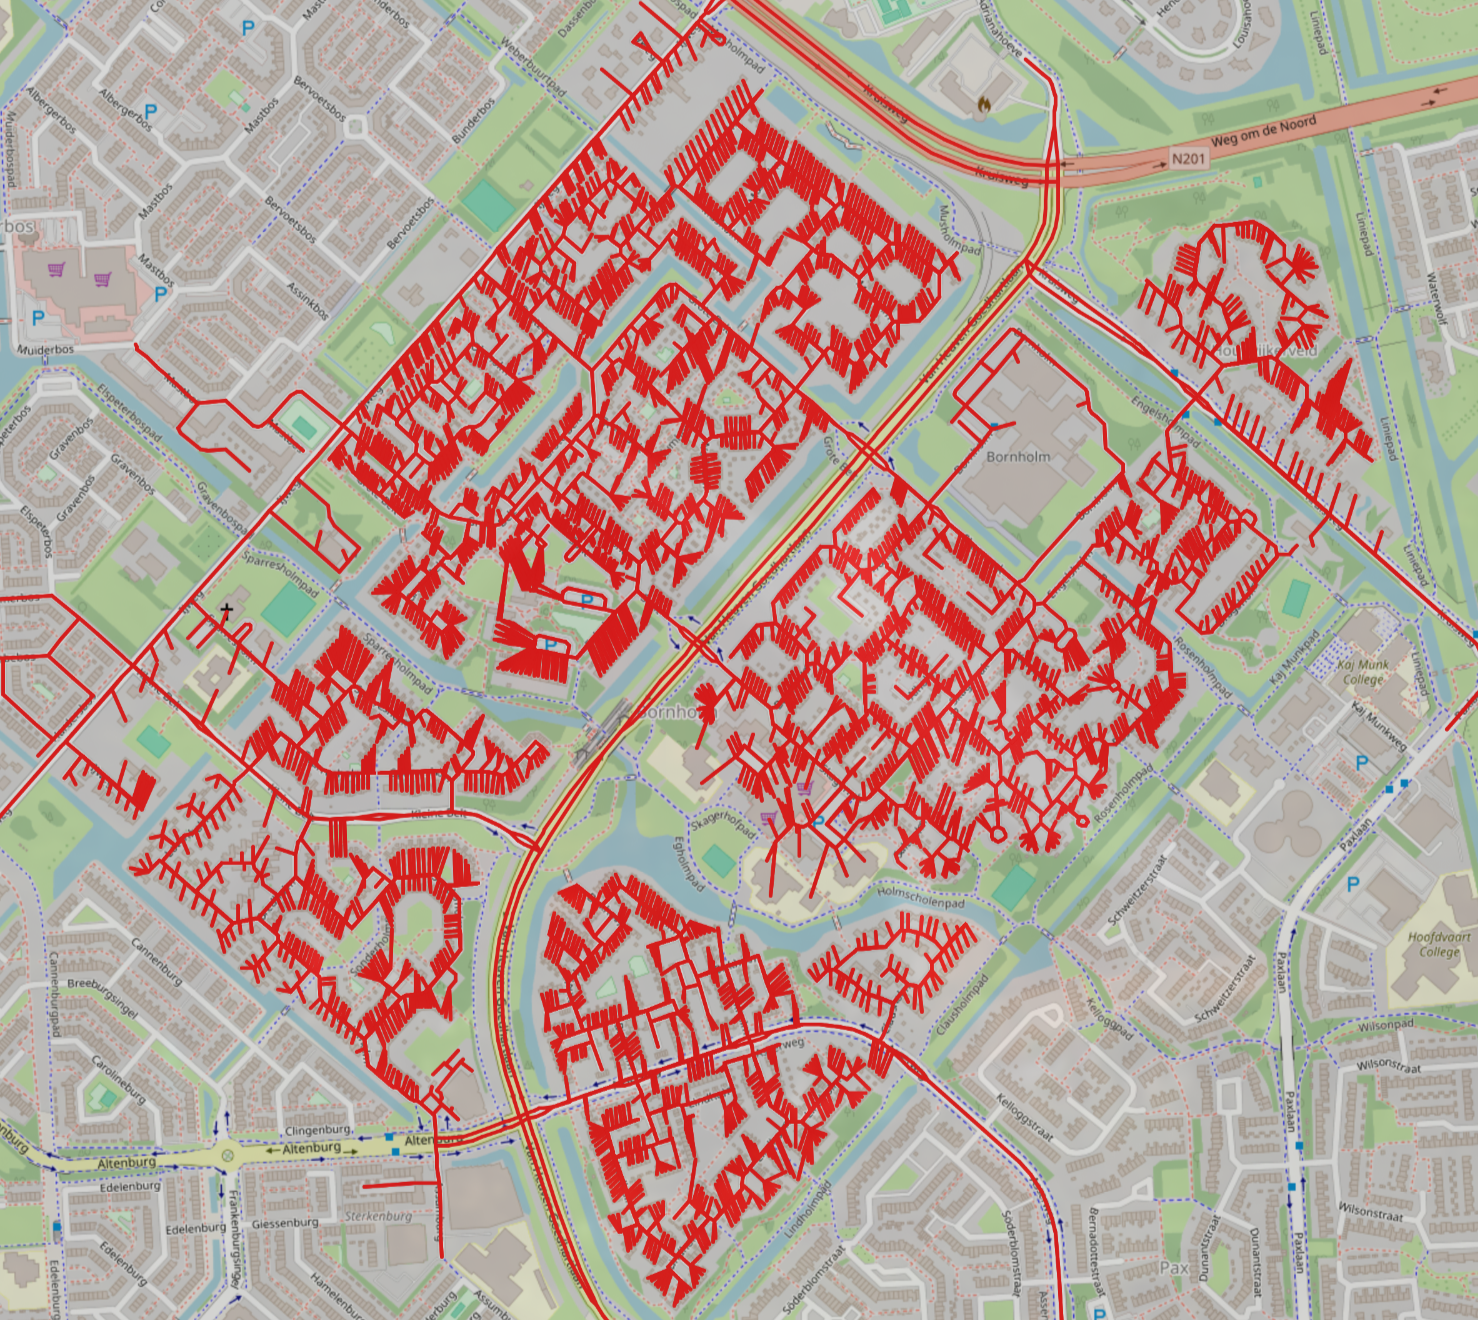
\includegraphics[width=\textwidth]{Pictures/Westeinde_quarter.png}
		\caption{Westeinde}
		\label{fig:Westeinde}
	\end{subfigure}
	\hfill
	\begin{subfigure}[b]{0.585\textwidth}
		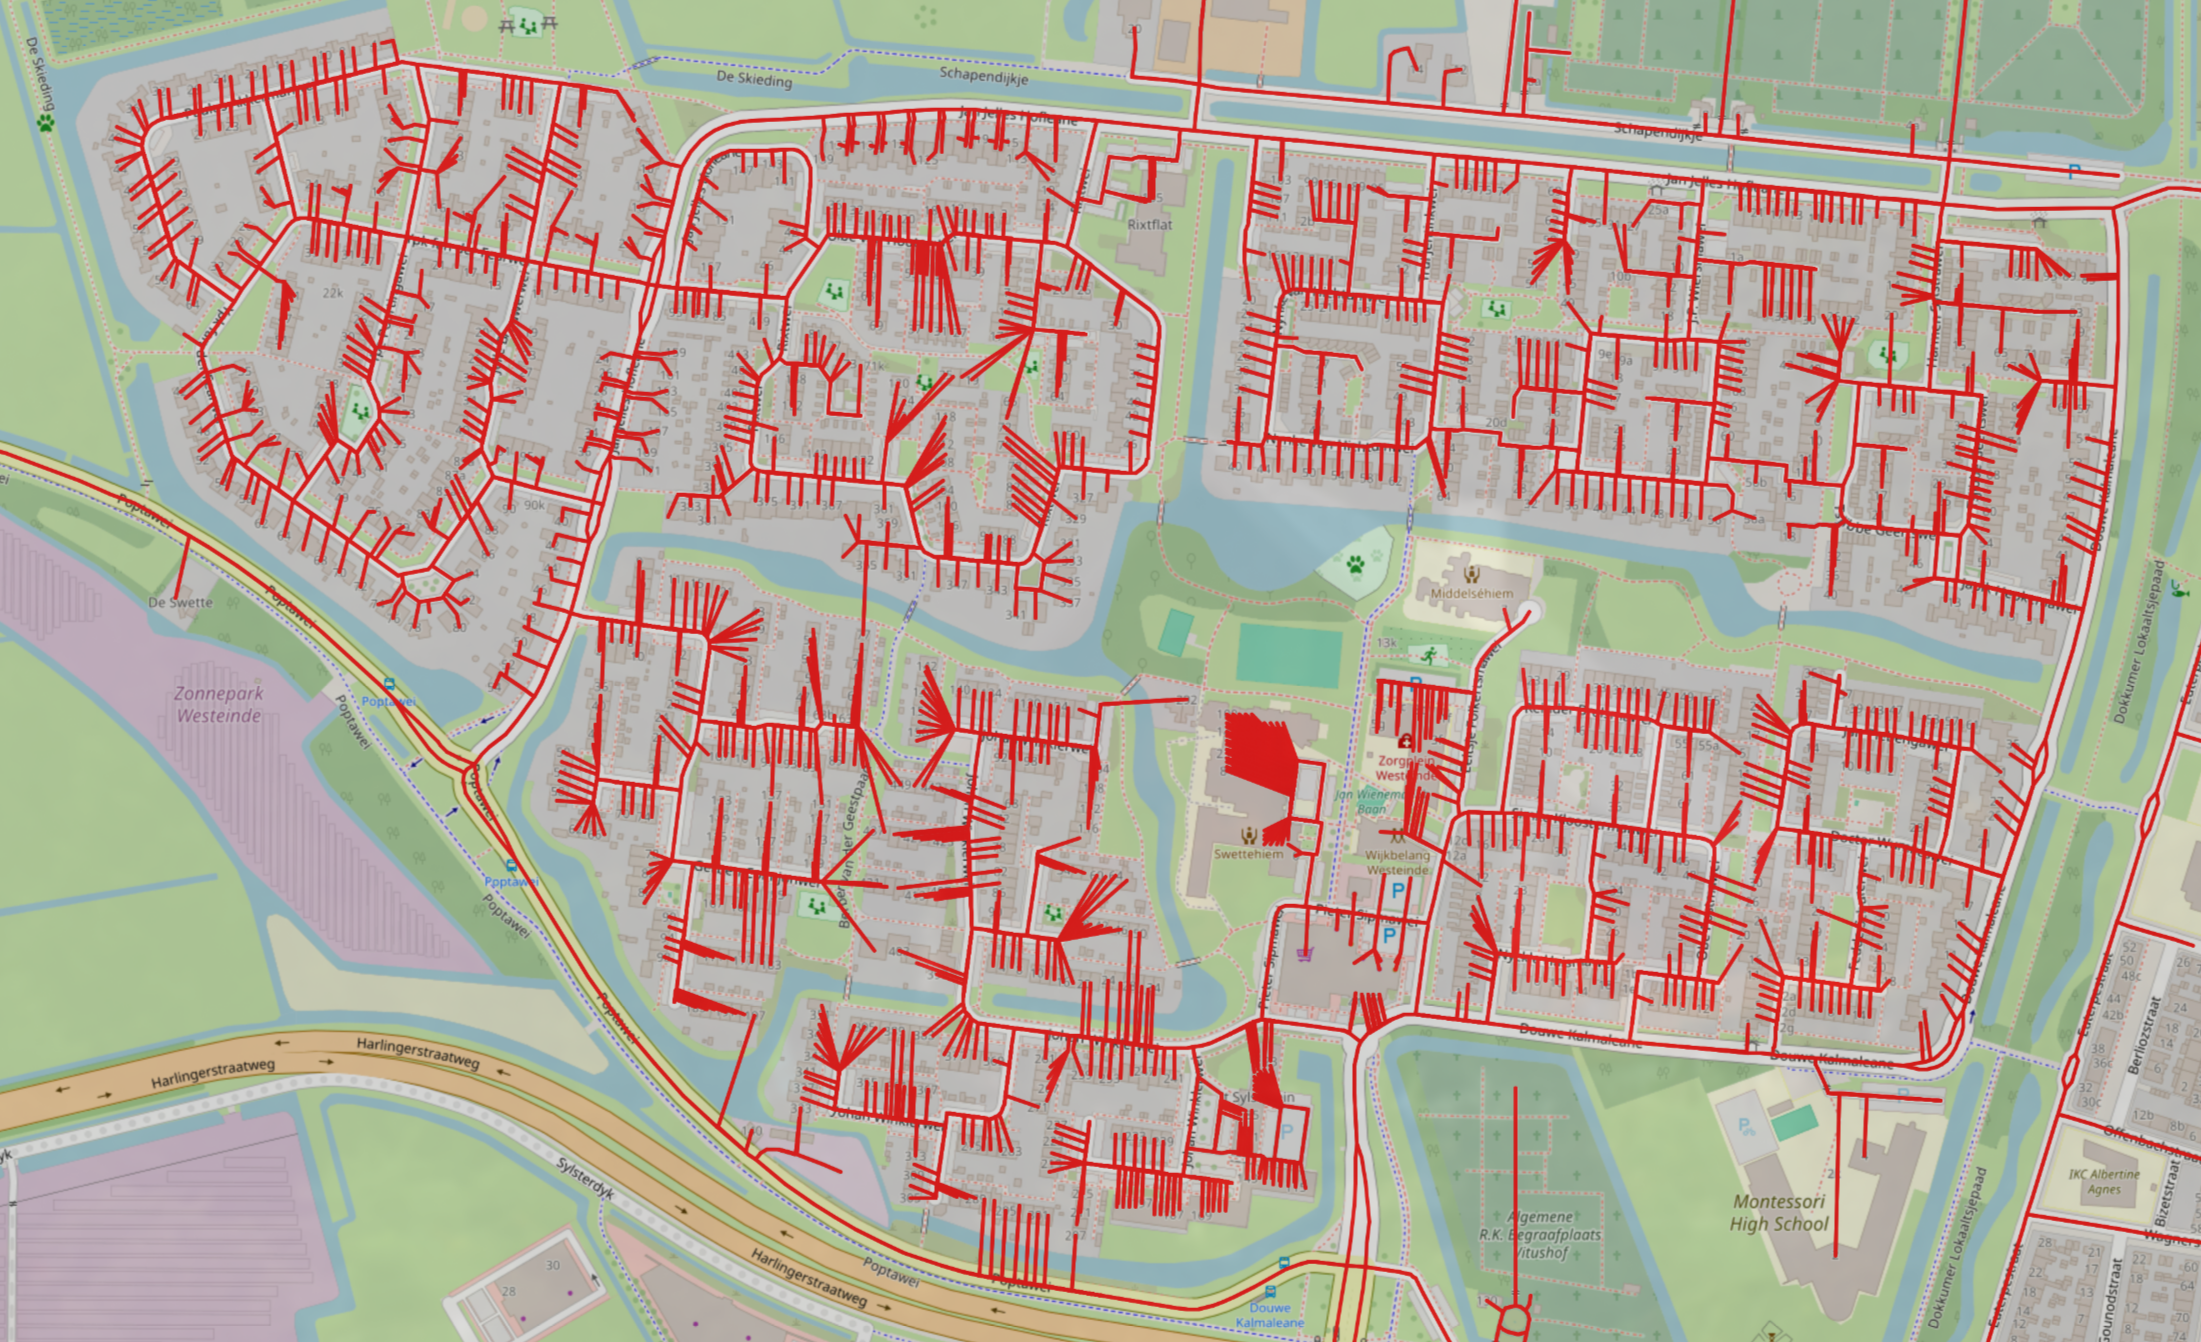
\includegraphics[width=\textwidth]{Pictures/Bornholm_quarter.png}
		\caption{Bornholm}
		\label{fig:Bornholm}
	\end{subfigure}
	\caption{Maps of the quarters Westeinde and Bornholm.}
	\label{fig:combined2}
\end{figure}
For these neighborhoods, there is still some variation around the fitted BHH formula, but Figure \ref{fig:combinedScatter2} shows vastly different
levels of variation, compared to Figure \ref{fig:combinedScatter}.
\begin{figure}[H]
	\centering
	\begin{subfigure}[b]{0.49\textwidth}
		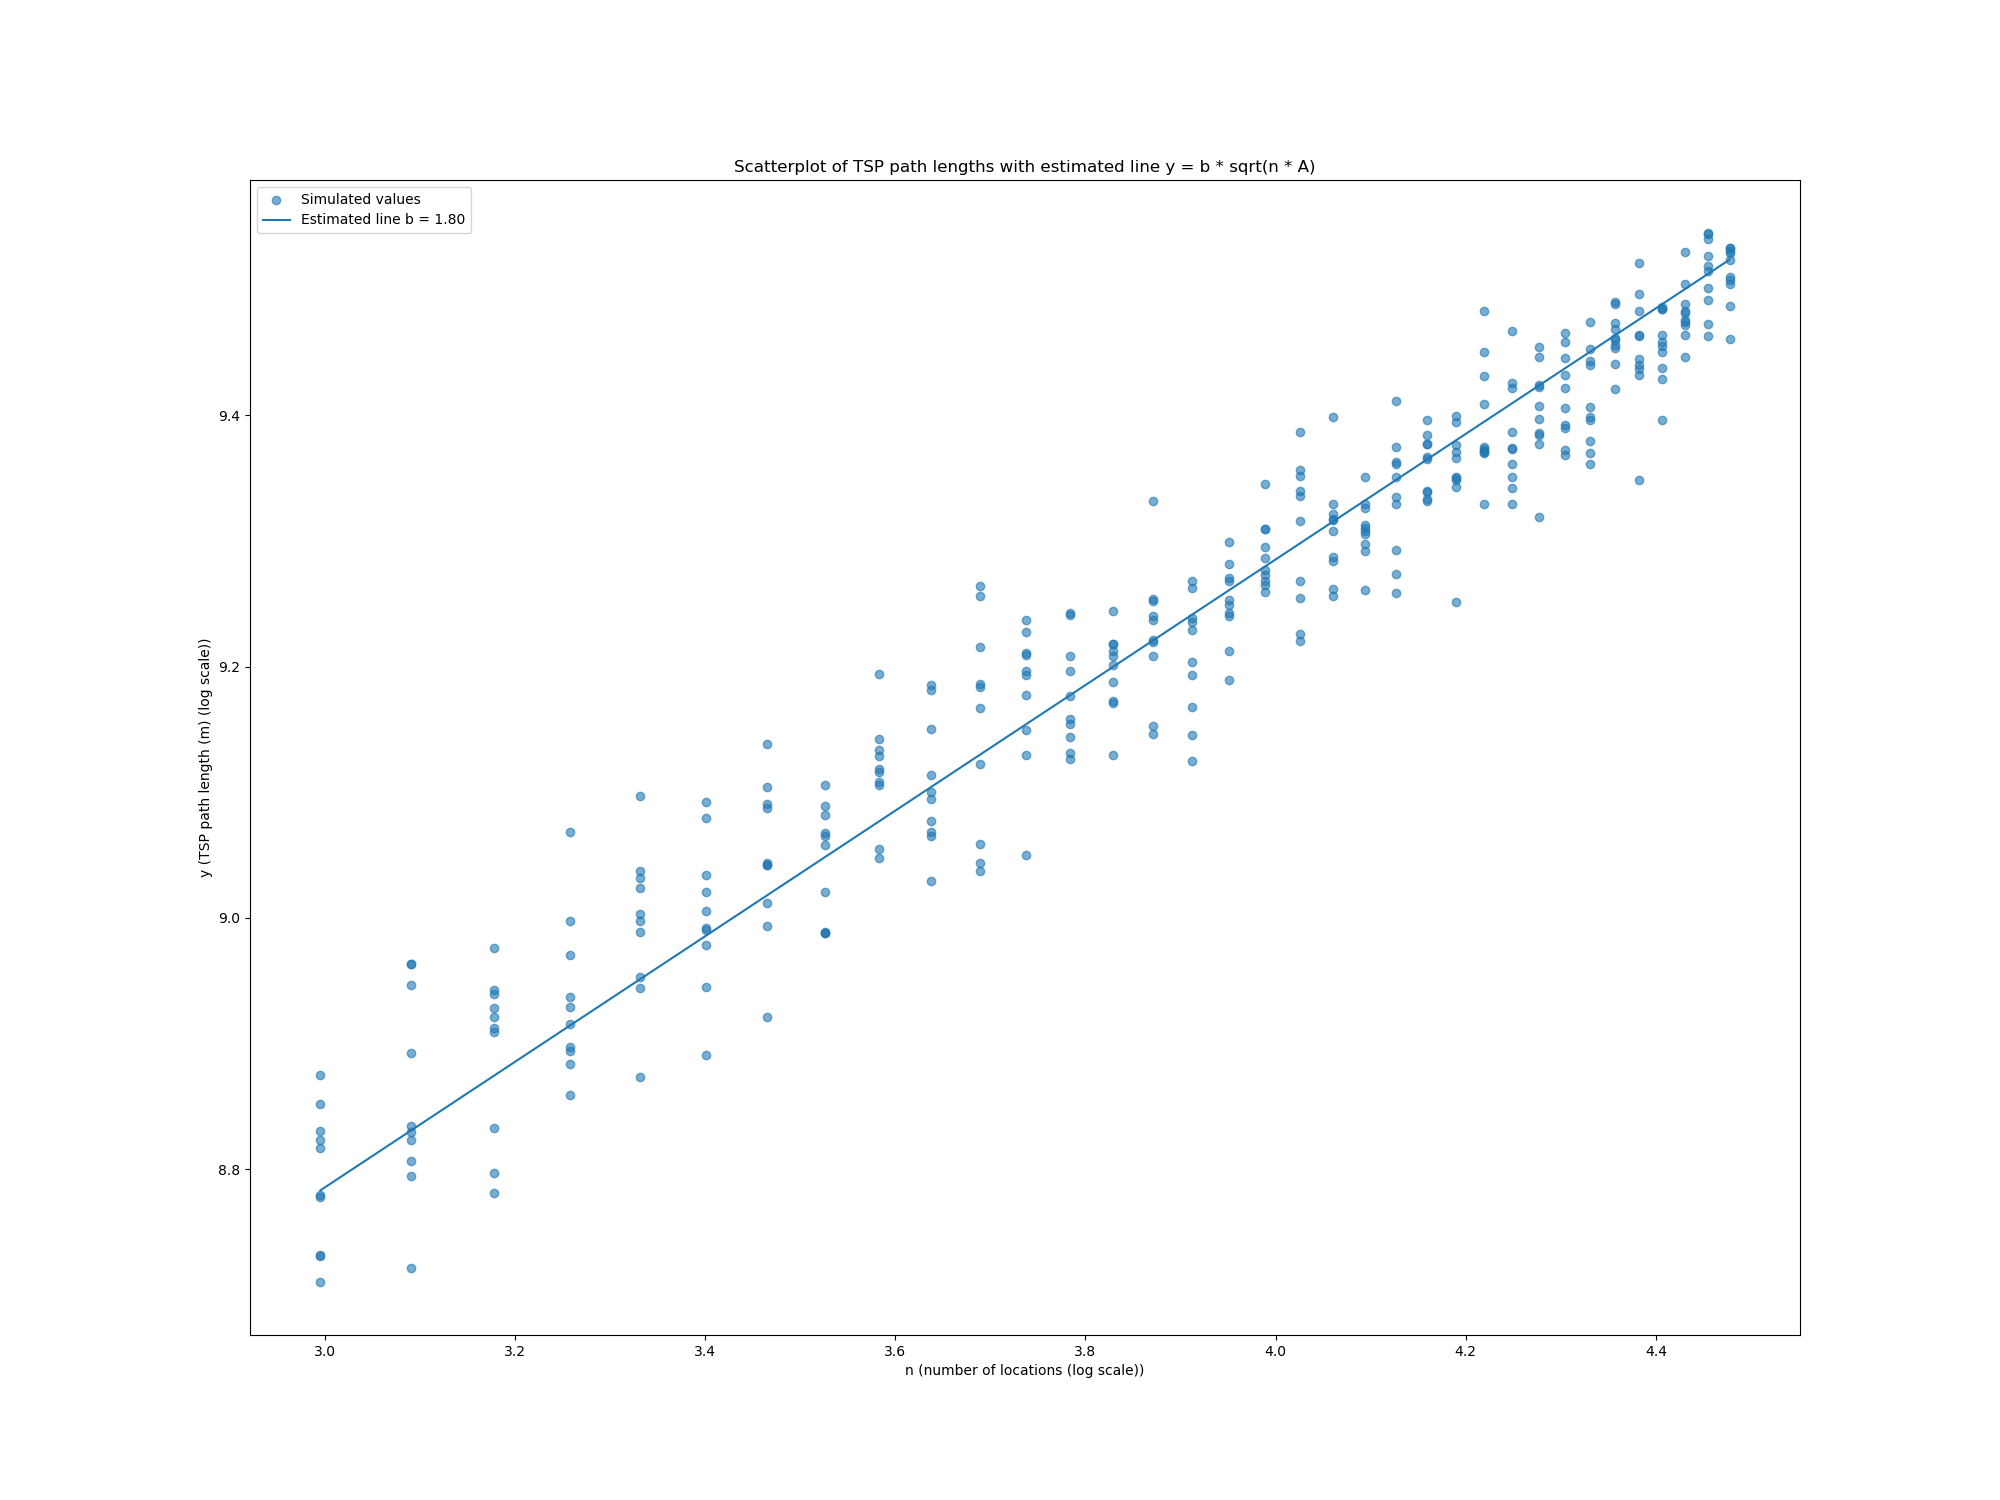
\includegraphics[width=\textwidth]{../project/plots/scatter_friesland-Westeinde.png}
		\caption{Schepenbuurt}
		\label{fig:WesteindeScatter}
	\end{subfigure}
	\hfill
	\begin{subfigure}[b]{0.49\textwidth}
		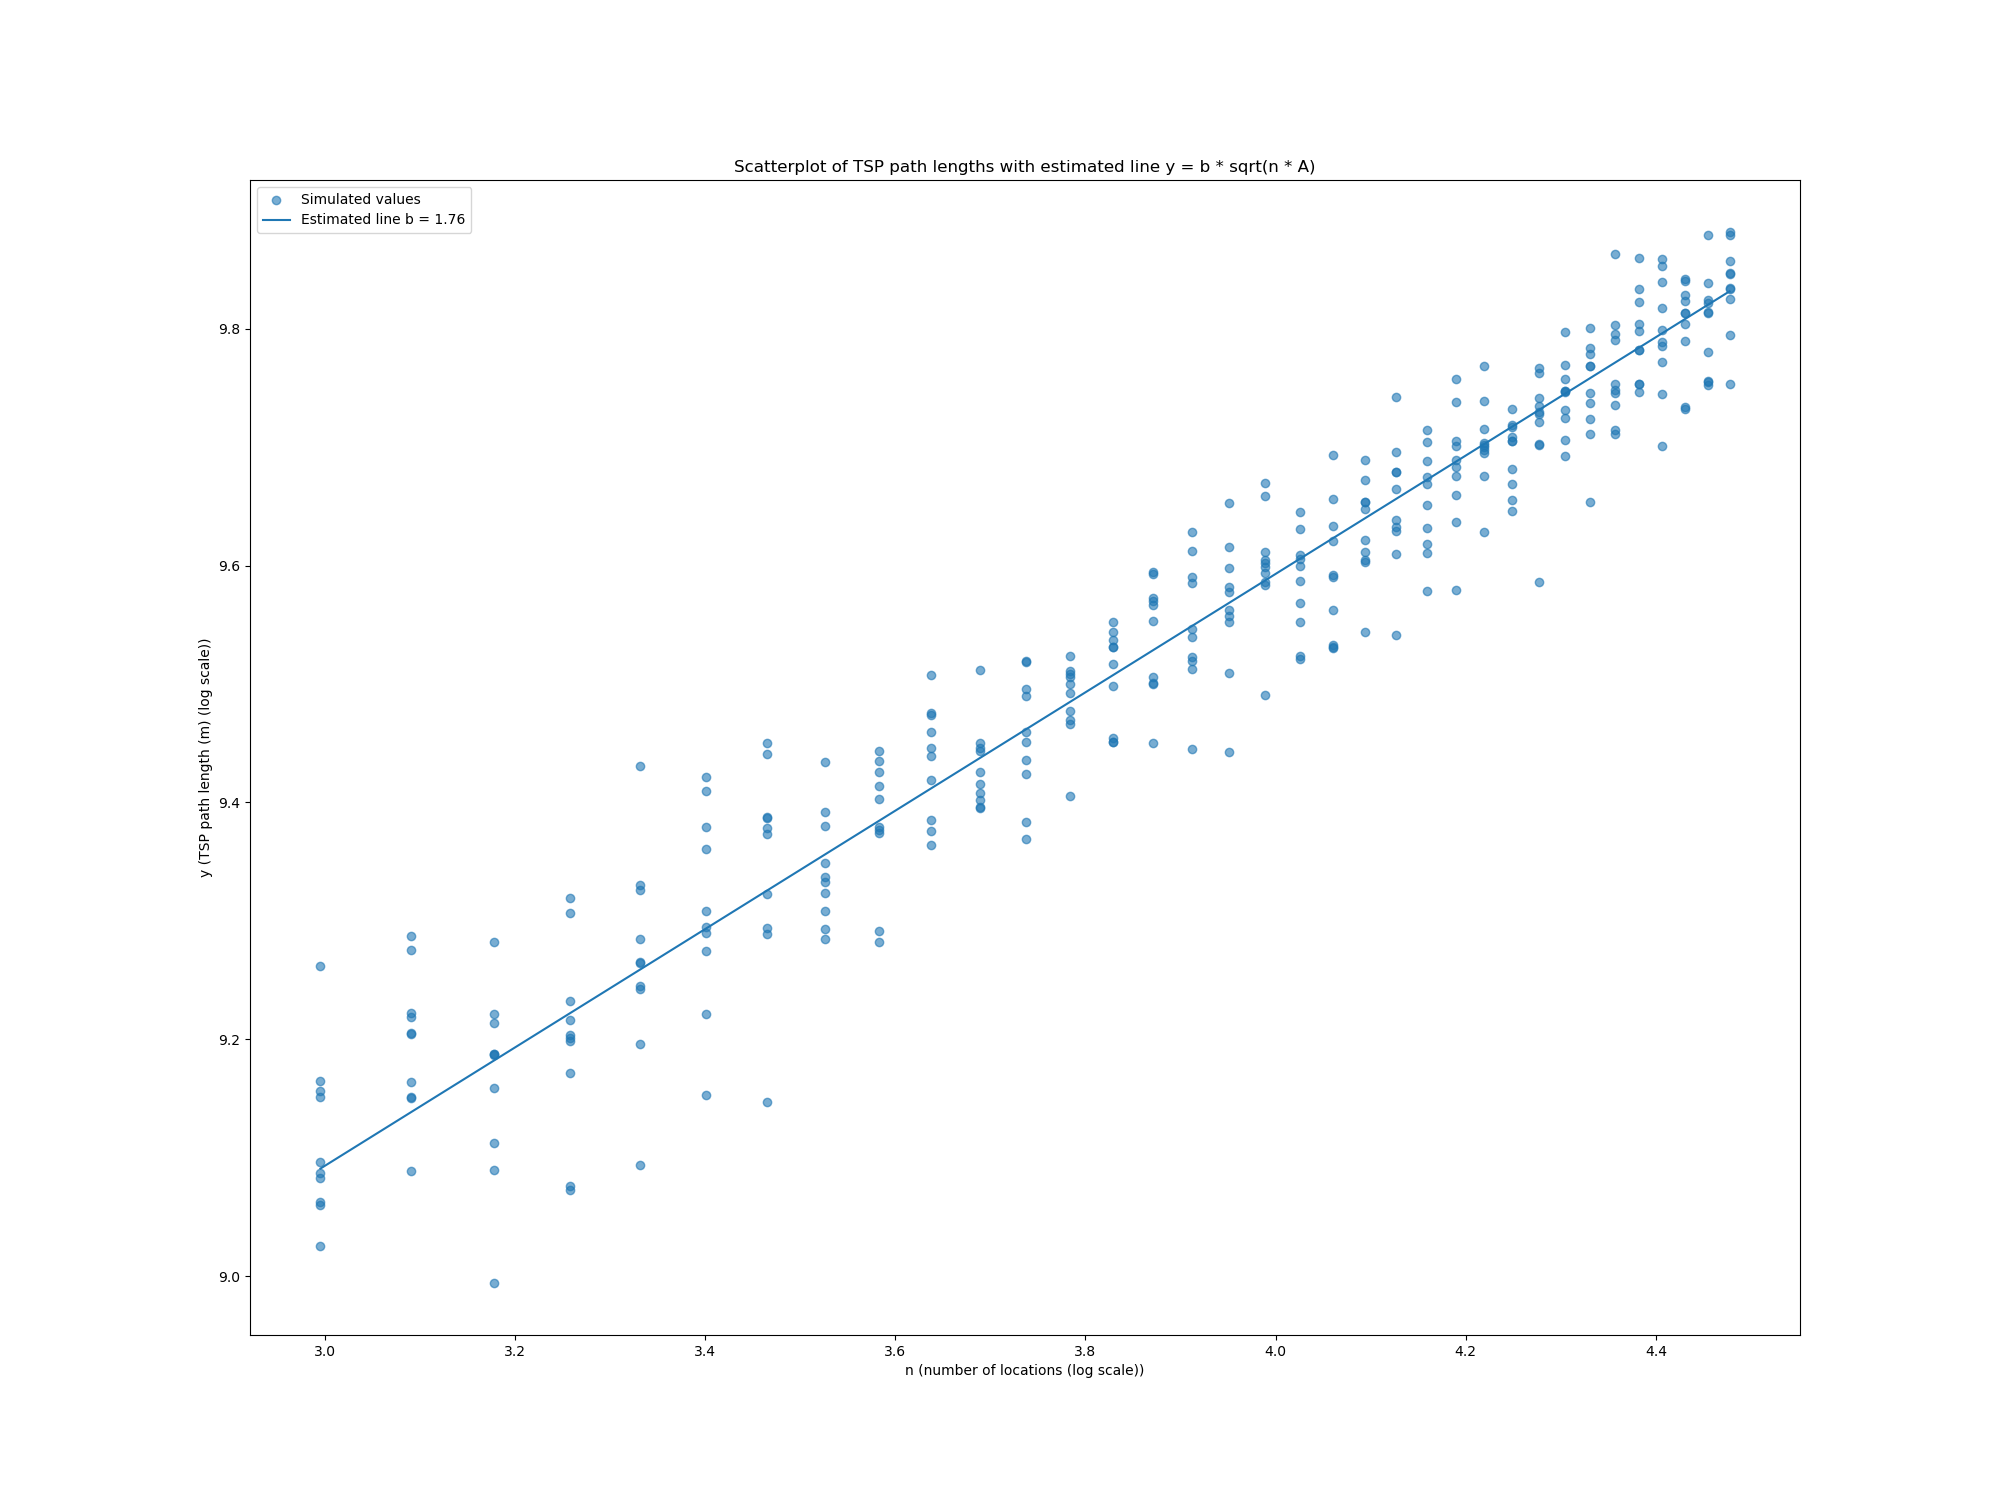
\includegraphics[width=\textwidth]{../project/plots/scatter_noord_holland-Bornholm.png}
		\caption{Stad van de Zon}
		\label{fig:BornholmScatter}
	\end{subfigure}
	\caption{Scatter plots of TSP path length vs number of locations for the quarters Westeinde and Bornholm (log-log scale).}
	\label{fig:combinedScatter2}
\end{figure}
